\documentclass[twocolumn]{aastex62}

\newcommand{\vdag}{(v)^\dagger}
\newcommand\aastex{AAS\TeX}
\newcommand\latex{La\TeX}
\usepackage{amsmath}
\usepackage{physics}
\usepackage{hyperref}
\usepackage{natbib}
\usepackage[T1]{fontenc}
\usepackage[english]{babel}
\usepackage[utf8]{inputenc}
\usepackage{wasysym}

\begin{document}

\title{\Large AST5220-Milestone III: Evolution of structure in the Universe}

\author{Nils-Ole Stutzer}

\begin{abstract}
    
    \textit{The codes for this paper can be found at:} \newline \url{https://github.com/SagittariusA-Star/AST5220-Milestones}
\end{abstract}

\section{Introduction} \label{sec:Intro}
Nowadays cosmology is considered a high precision field of science, a status which cosmology gained through high precision measurements of the Cosmic Microwave background (CMB) with several telescopes and probes, Planck \citep[]{planckcollaboration:2018} being the most significant to date. Planck's measurements of the CMB anisotropies have led to a revolution in cosmology, as the accurate measurements can be used to estimate cosmological parameters and subsequently tightly constrain cosmological models of the universe we live in.

In order to estimate cosmological parameters one needs to first model the CMB. This paper is a step towards the final goal of computing the angular CMB anisotropy power spectrum of temperature perturbations. We will continue the work of \cite{stutzer:2020a} and \cite{stutzer:2020b} by further building on the model of the universe by implementing the perturbations that ultimately form the anisotropies of CMB. We will do this by solving the couples set of differential equations (ODEs) of the multipole moments of the radiation (mainly photons), cold dark matter (CDM) and baryonic matter, neglecting neutrinos and the polarization of photons for simplicity. Also we only consider hydrogen to make up the baryons, an approximation which should hold fairly well, as hydrogen is the dominant species of baryons. These can subsequently be used to compute the theoretical CMB power spectrum for a set of cosmological parameters (future work).

\section{Method} \label{sec:Method}
The equations and relations presented here are, unless otherwise stated, provided by \cite{callin:2006}, \cite{winther:2020b} and or \cite{dodelson:2003}.

\subsection{The System of Equations} \label{subsec:system}
After having modeled the large scale evolution of the universe and its recombination history, we can add the small inhomogeneities of matter-energy of photons, CDM and baryonic matter and compute their evolution over time as a function of scale. The evolution of the perturbations for different scales are found by solving the linearized Einstein and Boltzmann equations with the initial conditions set up by inflation, which are derived in detail in \cite{dodelson:2003}. In principle this is merely a system of coupled ODEs which have to be solved for. However, there are some difficulties. Since the universe was hot and dense at early times, an electron would only "see" a short distance, and hence could only be affected by nearby temperature fluctuations. This is seen from the large optical depth at early times as found by \cite{stutzer:2020b}. Since the system was effectively in thermodynamic equilibrium with only small fluctuations, only the first few multipoles are relevant for the evolution of the photon-baryon plasma at early times. The relevant multipoles are the monopole $\Theta_0$ representing the average temperature of the electron, the dipole $\Theta_1$ which is a velocity term due to the doppler effect of the fluid and the quadrupole $\Theta_2$ which is the only relevant source for polarization this early on \citep[]{winther:2020b}. This early regime is called tight coupling, where matter and radiation forms a tightly coupled plasma.

Later on the universe became optically thinner and multipoles $\Theta_\ell$ of higher orders became relevant. In principle, since the ODEs for the multipoles of different order are all coupled, one needs to solve for a high number of these coupled equations. As this is highly inefficient, we make use of the line of sight integration developed by Zaldarriaga and Seljak, which only needs a few (six) of the multipoles. 

Since we, as mentioned in the Introduction, only consider photons, CDM and baryonic matter perturbations we get the following differential equations for the photon multipole moments

\begin{align}
    \Theta^\prime_0 &= -\frac{ck}{\mathcal{H}} \Theta_1 - \Phi^\prime, \\
    \Theta^\prime_1 &=  \frac{ck}{3\mathcal{H}} \Theta_0 - \frac{2ck}{3\mathcal{H}}\Theta_2 +
    \frac{ck}{3\mathcal{H}}\Psi + \tau^\prime\left[\Theta_1 + \frac{1}{3}v_b\right], \\
    \Theta^\prime_\ell &= \frac{\ell ck}{(2\ell+1)\mathcal{H}}\Theta_{\ell-1} - \frac{(\ell+1)ck}{(2\ell+1)\mathcal{H}}
    \Theta_{\ell+1} \nonumber \\
    &+ \tau^\prime\left[\Theta_\ell - \frac{1}{10}\Pi
    \delta_{\ell,2}\right], \qquad  2 \le \ell \leq \ell_{\textrm{max}} \\
    \Theta_{\ell}^\prime &= \frac{ck}{\mathcal{H}}
    \Theta_{\ell-1}-c\frac{\ell+1}{\mathcal{H}\eta(x)}\Theta_\ell+\tau^\prime\Theta_\ell,
    \quad\quad \ell = \ell_{\textrm{max}},
\end{align}
The first two moments of which can be thought of as the density and the velocity perturbation respectively. We let $\ell_\mathrm{max} = 5$ for a total of six multipole moments for photons. The scaled Hubble parameter $\mathcal{H}$ and the conformal time $\eta$ are computed in \cite{stutzer:2020a}, and the optical depth $\tau$ and its derivative $\tau^\prime$ are computed in \cite{stutzer:2020b}. The polarization tensor $\Pi = \Theta_2$ if polarization is neglected. The scale, of which every perturbation is a function of, is given by the wavenumber $k$ and the light speed is $c$ (all units are in the SI system). 

The perturbations to the CDM and baryonic matter-energy field are given by 
\begin{align}
    \delta_{\rm CDM}^\prime &= \frac{ck}{\mathcal{H}} v_{\rm CDM} - 3\Phi^\prime \\
    v_{\rm CDM}^\prime &= -v_{\rm CDM} -\frac{ck}{\mathcal{H}} \Psi \\
    \delta_b^\prime &= \frac{ck}{\mathcal{H}}v_b -3\Phi^\prime \\
    v_b^\prime &= -v_b - \frac{ck}{\mathcal{H}}\Psi + \tau^\prime R(3\Theta_1 + v_b),
\end{align}
where the density perturbations for CDM and baryons are given by $\delta_\mathrm{CDM}$ and $\delta_b$ respectively being the monopole moment of the matter components. The dipole moment of perturbations of the two matter components, i.e. the velocity perturbations are given by $v_\mathrm{CDM}$ and $v_b$. The factor $R = \frac{3\Omega_{r,0}}{4\Omega_{b,0}a}$, where $a$ is the scale factor.

And finally the perturbations to the time and space components of the metric (in the Newtonian gauge) are given as 
\begin{align}
    \Phi^\prime &= \Psi - \frac{c^2k^2}{3\mathcal{H}^2} \Phi
    + \frac{H_0^2}{2\mathcal{H}^2}
    \bigl[\Omega_{\rm CDM,0} a^{-1} \delta_{\rm CDM}\\
    & + \Omega_{b,0} a^{-1} \delta_b + 4\Omega_{r,0}
    a^{-2}\Theta_0 \bigr] \\
    \Psi &= -\Phi - \frac{12H_0^2}{c^2k^2a^2}\left[\Omega_{r,0}\Theta_2\right].
\end{align} 
Through Einsteins field equations one can see that the matter-energy content of the universe and the space-time curvature are determined by each other, and hence the perturbations of the matter-energy components (photons, CDM and baryons) will result in these metric perturbations. 
Note that in fact only one of the two metric perturbations is dynamical, meaning we don't have to solve for $\Psi$ as an ODE as it is determined by $\Phi$ directly.
Because these metric perturbations are perturbations to the curvature of space-time caused by the presence of a matter-energy perturbation, they will define the gravitational potential wells that matter and radiation can fall into or oscillate in. 

As mentioned before there is however a slight complication in that the universe is hot and dense in the beginning, with a tight coupling between matter and radiation. In the tightly coupled regime $\tau'$ is large and $\Theta_1$ and $v_b$ are close to zero. Thus the factor $\tau' (3\Theta_1 + v_b)$ becomes numerically very unstable early on. Therefore one needs to do an approximation, explained in detail by \cite{callin:2006} or \cite{winther:2020b}, where we define the term 
\begin{align}
q &= \bigr(-[(1-R)\tau^\prime + (1+R)\tau^{\prime\prime}](3\Theta_1+v_b) \\&-
            \frac{ck}{\mathcal{H}}\Psi + (1-\frac{\mathcal{H}^\prime}{\mathcal{H}})\frac{ck}{\mathcal{H}}(-\Theta_0 +
            2\Theta_2) \\ &- \frac{ck}{\mathcal{H}}\Theta_0^\prime\bigr)/\bigl((1+R)\tau^\prime + \frac{\mathcal{H}^\prime}{\mathcal{H}} -
            1\bigr)
\end{align}
which is used to get more numerically stable expressions given as 
\begin{align}
    v_b^\prime &= \frac{1}{1+R} \left[-v_b - \frac{ck}{\mathcal{H}}\Psi + R(q +
    \frac{ck}{\mathcal{H}}(-\Theta_0 + 2\Theta_2) - \frac{ck}{\mathcal{H}}\Psi)\right]\\
    \Theta^\prime_1 &= \frac{1}{3} (q - v_b^\prime).
\end{align}
The ODEs for the monopole $\Theta_0$, as well as for $\delta_\mathrm{CDM}$, $v_\mathrm{CDM}$ and $\delta_b$ in the tightly coupled regime are simply the same as outside tight coupling as defined earlier.
Apart from the above rewriting for numerical stability sake, the only difference from the full equations valid outside of tight coupling, is that one only needs to solve ODEs for the first two multipole moments $\Theta_0$ and $\Theta_1$ (and the CDM and baryonic quantities) since all other $\Theta_\ell$ are directly determined by the two former. Specifically without considering polarization the multipoles are given by
\begin{align}
    \Theta_2 &= 
    -\frac{20ck}{45\mathcal{H}\tau^\prime} \Theta_1, \quad\quad \textrm{(without polarization)}\\ 
    \Theta_\ell &= -\frac{\ell}{2\ell+1} \frac{ck}{\mathcal{H}\tau'} \Theta_{\ell-1}, \quad\quad \ell > 2.
\end{align}
Now that all equations for the tightly coupled regime are set up, we only need initial conditions before solving the system of ODEs in this regime. The initial conditions are set up by inflation an are as shown in \cite{winther:2020b} given by 

\begin{align}
    \Psi &= -\frac{2}{3}\\
    \Phi &= -\Psi \\
    \delta_{\rm CDM} &= \delta_b = -\frac{3}{2} \Psi \\
    v_{\rm CDM} &= v_b = -\frac{ck}{2\mathcal{H}} \Psi\\
    \Theta_0 &= -\frac{1}{2} \Psi \\
    \Theta_1 &= +\frac{ck}{6\mathcal{H}}\Psi \\
    \Theta_2 &= 
    -\frac{20ck}{45\mathcal{H}\tau^\prime} \Theta_1, \quad\quad \textrm{(without polarization)}\\
    \Theta_\ell &= -\frac{\ell}{2\ell+1} \frac{ck}{\mathcal{H}\tau^\prime} \Theta_{\ell-1}.
\end{align}
In fact due to the system of equations being linear means that one can later pick a different initial condition for $\Psi$, and simply propagate the change through the others if other normalizations are desired. 

To integrate the perturbations over the entire history of the universe through today, we must finally determine how to transition from the system of the tightly coupled regime to the full set of equations. The time $x_\text{end of tc}$ of transition is essentially when $|\dv{\tau}{x}| < 10 \cdot \mathrm{min}(1, \frac{ck}{\mathcal{H}})$ but no later than the very beginning of recombination at $z\approx 1700$ which corresponds to $X_e\approx 0.999$ from \cite{winther:2020b}.

After determining the time of transition, initial conditions for the full system are needed in order to solve the ODEs. These initial conditions are simply the values of the quantities at the time right before transition, i.e. the last values in the regime of tight coupling. 

Some of the things we expect to see in the final solutions are the monopole moment of the photon(-baryon plasma) to oscillate in the gravitational potentials before decoupling happens. This is the interplay between the radiation pressure expanding a perturbation and gravity pulling collapsing it, together forming an oscillatory interplay. After matter and radiation decouple, the photons can free-stream, and the perturbations are frozen in on the surface of last scattering as the CMB anisotropies. Further more, due to the presence of baryons in the primordial plasma we expect the oscillations to be asymmetric, as baryons tend to clump more than they ... Generally we also expect different scales to perform differently, as small scales well below the sound horizon (the scale a sound wave can have traveled at a given time) at decoupling $r_* = \int^{\eta_*}_0 c_s d\eta$, for sound speed $c_s$, have the chance to performed more oscillations than scales just barely within the sound horizon. Scales above the sound horizon have not even had the chance to perform a single oscillation within the time of decoupling.

The matter density perturbations $\delta$ should reproduce the known plots of the Meszaros suppression, where the perturbations grow as the scale factor $a$ squared prior to matter-radiation equality $a_\text{eq}$, while being suppressed to grow as $\ln a$ after entering the horizon prior to $a_\text{eq}$. After $a_\text{eq}$ we then expect to see perturbations to grow proportional to the scale factor. Further we expect to see the smaller perturbations to enter the horizon earlier, hence the large scales (i.e. larger k) should be suppressed more.

The scale dependence of the metric perturbations should also be seen. Prior to horizon entry the potentials $\Phi$ and $\Psi$ should start out equally in size bu with opposite signs. They should behave as constants when outside the causally connected horizon defined by the Hubble sphere. When entering the horizon, the whole perturbation is causally connected, and the expanding universe will lead to the potential wells given by $\Phi$ and $\Psi$ to "flatten", reducing the well's "depth". This is sean by $\Phi$ and $\Psi$ decaying, symmetrically, towards zero after entering the horizon. And again the smaller scales are entering the horizon earlier resulting metric perturbations of larger $k$ to decay first, and the super horizon perturbations to decay slowly or not at all. 

These are just some of the expectations to look out for, but there could of course be more interesting things to discover in the final results.




\subsection{The Implementation} \label{subsec:implementation}
Now that the system of ODEs is set up, we are ready to solve it using C++. The main idea of solving is that we want to loop through different scales $k$ and for each iteration solve the system of ODEs through time $x$. We use logarithmically spaced values for the wavenumbers $k$ to loop through. Inside each iteration of the $k$-loop we fist find the time $x_\text{end of tc}$ when tight coupling ends. This time is used to divide the time line $x$ into two, one for each regime. In the first regime the initial conditions are set at described in \ref{subsec:system} as set up by inflation. The ODEs for tight coupling are solved and the quantities depending on those (i.e. the higher order multipoles) are computed, after which the results are saved in $n_x\times n_k$ matrices for later use.

Similarly the second half of the time axis, after transitioning outside the tight coupling, the full system of ODEs are solved with the initial conditions being the last values of tight coupling. The results are subsequently saved in the $n_x\times n_k$ grid matrices. The system of ODEs in each regime is solved using the \texttt{ODEsolver}-routine provided by \cite{winther:2020b}. The reason for dividing the ODE system in two, instead of solving the whole system in on go, is that the number of dynamical equations (i.e. ODEs) is different in the two regimes. Hence two separate ODE objects are needed for solving. 

Finally, before plotting the final outputs, spline interpolations of the saved $n_x\times n_k$ grid values of the solved quantities are made, so as to make a more continuos representation of each quantity. For that the \texttt{Spline2D}-routine by \cite{winther:2020b} is used. The very final output for plots are solved in data files, and plots are made in Python.



\begin{figure*}
    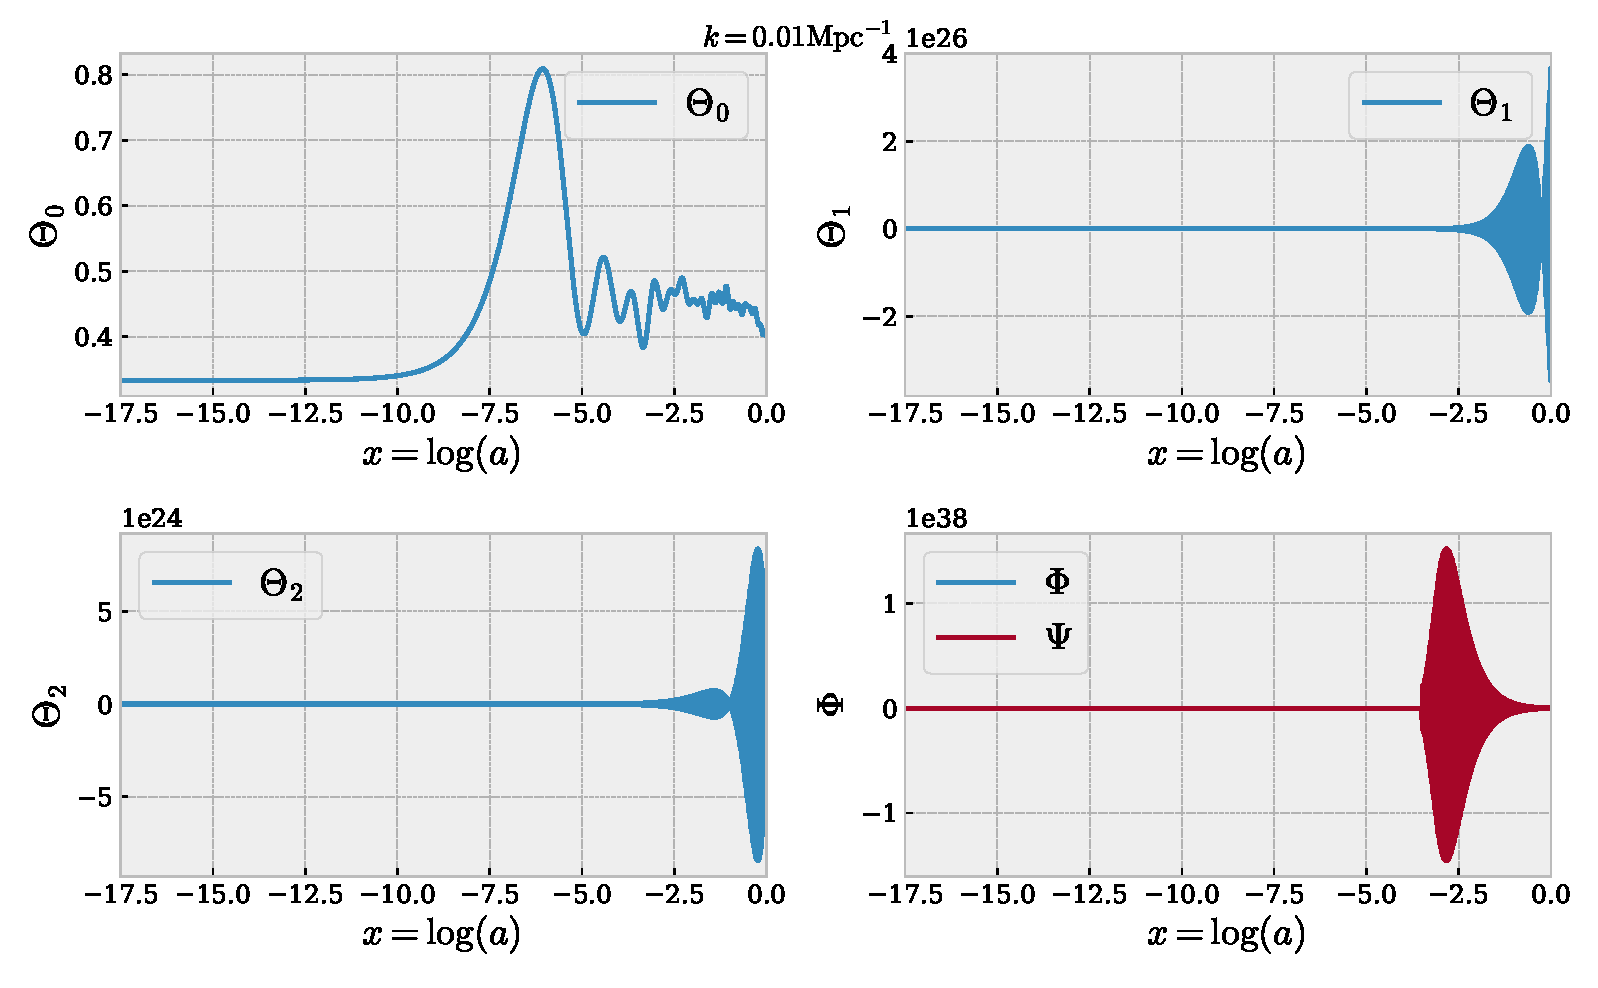
\includegraphics[scale = 0.65]{Figures/fig1.pdf}
    \caption{The figure shows (\textbf{Upper left}) the monopole moment $\Theta_0 = \frac{1}{4}\delta_\gamma$ and (\textbf{upper right}) the dipole moment $\Theta_1 = -\frac{1}{3}v_\gamma$, roughly corresponding to the density and velocity perturbation of radiation energy-density perturbation respectively. Also shown (\textbf{lower right}) are the metric perturbations $\Phi$ and $\Psi$ in the Newtonian gauge. All quantities plotted are functions of the log-scale factor $x = \ln a$ and scale $k$, and are shown for several different wavenumbers. The background color marks the epoch of dominance; yellow, blue and purple represent radiation, matter and dark energy dominated epochs respectively. The red background color corresponds to the epoch of recombination, given by the width of the peak of the visibility function from \cite{stutzer:2020b}.} 
    \label{fig:fig1}
\end{figure*}

\begin{figure*}
    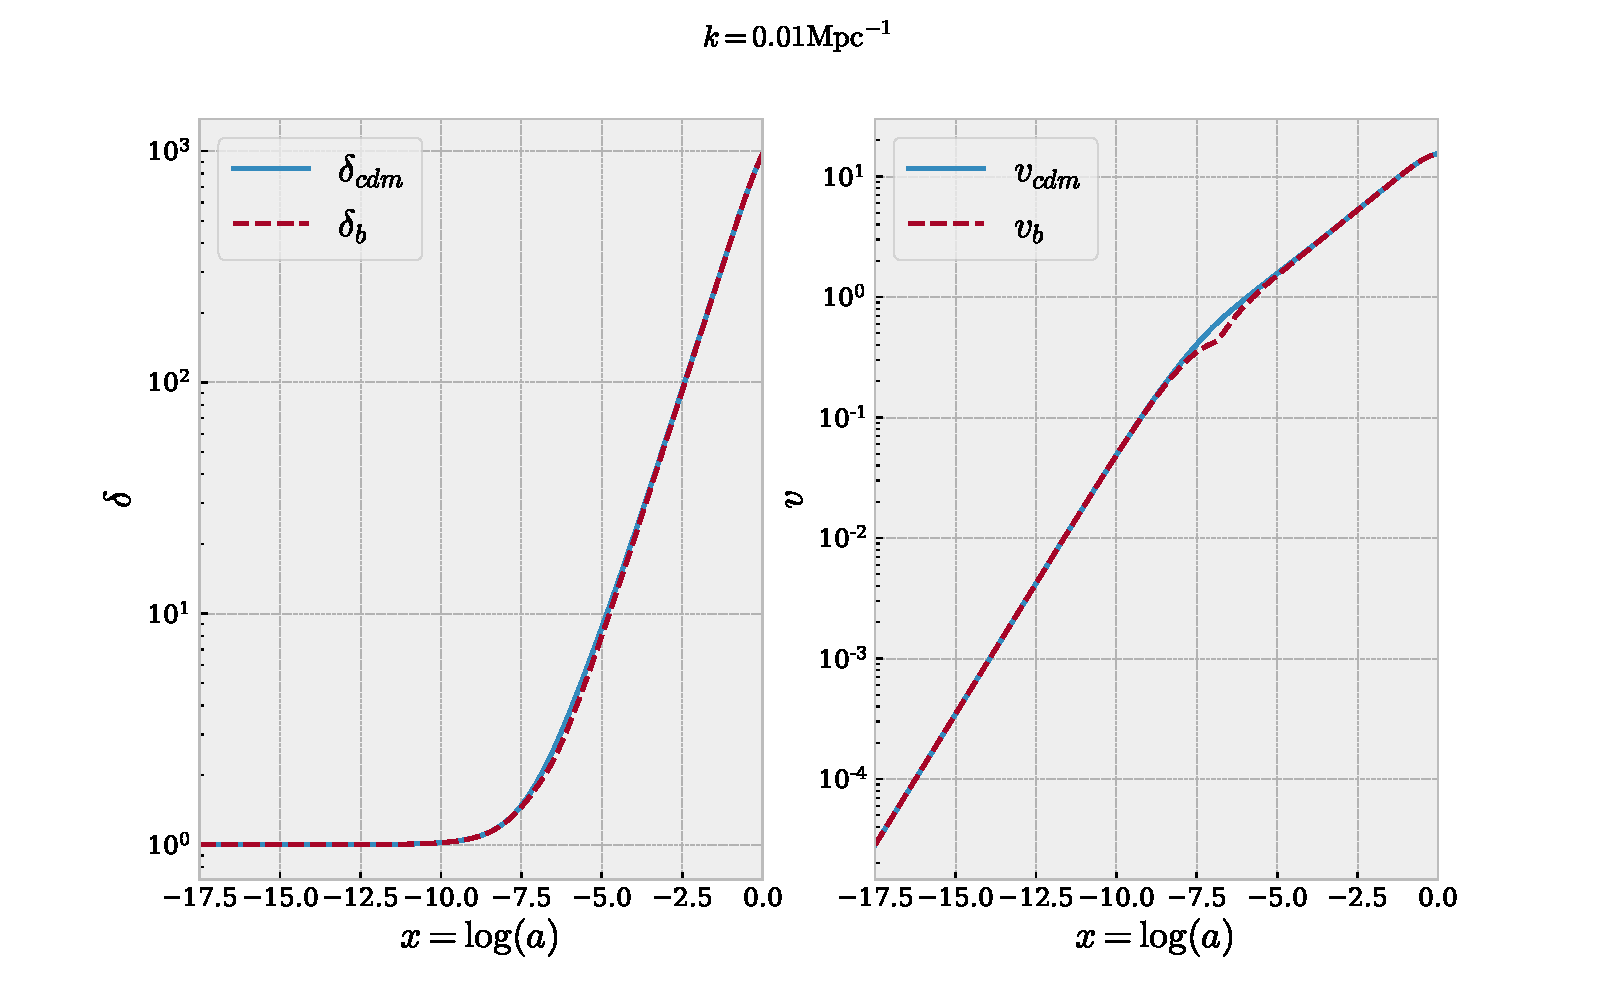
\includegraphics[scale = 0.65]{Figures/fig2.pdf}
    \caption{The left panel shows the density perturbations of the dark and baryonic matter perturbations (solid and dashed lines respectively). The right panel shows the velocity perturbations for dark and baryonic matter (same meaning of line style as in the left panel). The quantities shown are functions of the log-scale $x = \ln a$ and scale, and are plotted for several wavenumbers $k$.  The background color marks the epoch of dominance; yellow, blue and purple represent radiation, matter and dark energy dominated epochs respectively. The red background color corresponds to the epoch of recombination, given by the width of the peak of the visibility function from \cite{stutzer:2020b}.}
    \label{fig:fig2}
\end{figure*}


\section{Results/Discussion}\label{sec:Results}

After having run the simulation computing the perturbations evolution throughout time, we end up with the plots seen in Figure \ref{fig:fig1} and Figure \ref{fig:fig2}.

In Figure \ref{fig:fig1} one can see the first two multipole moments $\Theta_0$ and $\Theta_1$ of the photon perturbations in the upper panels, as well as the two metric perturbations in the lower panel, all as functions of the log-scale factor $x$. In the lower panel the time and space components of the metric perturbations are marked with solid and dashed lines respectively. In each plot one can see the evolution of the respective quantity for six different scales, given by the wavenumber $k$ in the legend, spanning from sub to superhorizon scales. The color code in the background represent the respective epochs of dominance (i.e. radiation, matter and dark energy eras, see caption for details) as well as the epoch of recombination. The width of the latter one corresponds roughly to the width of the peak of the visibility function computed in \cite{stutzer:2020b}. 

In Figure \ref{fig:fig2} we see the density perturbations of the CDM and baryon components of the matter in the right panel and the corresponding velocity perturbations. Again the CDM and baryon graphs are marked with solid an dashed lines respectively. The same six wavenumbers are used to produce these results as for the ones presented in Figure \ref{fig:fig1}. The same color code used in Figure \ref{fig:fig1} is used in Figure \ref{fig:fig2}. 

Note that all quantities shown are in Fourier space, not position space. Hence the velocity perturbations of the matter components can actually be greater than unity, as they are not directly to interpret as the real space velocities.

\section{Discussion}\label{sec:Discussion}
When looking at the plots of the upper two panels in Figure \ref{fig:fig1} we see the monopole and dipole moments of the radiation perturbations. In fact early on, when baryons and photons where coupled, these two components formed a single fluid. When looking at, for instance, the monopole moment of the upper right panel, we see also the different behaviour of the perturbations on different scales. The largest scales, larger than the horizon at matter-radiation equality $k\ll k_\text{eq}$, stretching outside the Hubble sphere $r = c/H$, remain basically unaffected for the entire history of the universe. That is because the perturbations are larger than the causally connected region on which gravity and pressure could act, resulting in no growth or decrease in density or velocity as long as it hasn't entered.

On the very small scales smaller than the horizon at matter-radiation equality$k \gg k_\text{eq}$, e.g. $k = 0.3 /\mathrm{Mpc}$ and $0.0527 /\mathrm{Mpc}$ (see yellow and black curves), the behaviour of perturbations looks quite different. Prior to horizon entry (the times of entry is marked by the dotted vertical line for a given scale) the large and small scale modes behave the same, just being constant. However, once entering the horizon prior to equality, we see $\Theta_0$ behaves highly oscillatory. These oscillations are the so called acoustic oscillations of the matter-radiation plasma (as matter and radiation are highly coupled prior to recombination). The oscillations basically show the interplay between gravity, which contracts the perturbations rarifying them, and the pressure forces by the enormous radiation pressure expanding the perturbations. Once having enterd the horizon a perturbation grows rapidly, i.e. the density given by the monopole $\Theta_0$ grows when the perturbation accretes more plasma falling into the gravitational well set up by the perturbation. When the plasma falls in to the potential well, the radiation pressure increases, gradually slowing down the growth in $\Theta_0$, eventually able to counteract the pull of gravity completely. This expansion leads to the perturbation shrinking in density again. Once the blob has expanded it cools down, and the whole cycle starts over again resulting in the oscillatory behaviour seen. This is basically how sound waves in the primordial photon-baryon plasma look like in Fourier space.

The oscillations or relativistic sound waves on these small scales keep on going until the epoch of recombination. At that time the radiation and baryon decouple and the photons can free stream out of any potential wells. Thus the oscillations effectively stop as the photons travel freely, not being bound in the dense plasma. We see exactly this happening in the plots, where the oscillating perturbations decay rapidly as they cross the epoch of decoupling. Further more, it is these free streaming photons that give rise to the CMB we see today. Hence the anisotropies seen in the CMB are the frozen-in picture of the photons at their last oscillation before decoupling. In fact the perturbations that perform one half expansion, i.e. collapse to the point right before subsequent expansion, within the time of recombination $x_*$ form the first peak of the acoustic oscillation pattern in the later-to-be computed CMB angular power spectrum. This corresponds about to the $k = 9.24\cdot 10^{-3}/\mathrm{Mpc}$ scale monopole in our case (in fact slightly lower scale, but as seen in the plot this is the closest one we have computed). Similarly the other peaks of the CMB power spectrum are perturbations having performed multiples or halves of oscillations at the time of decoupling, and the troughs of the power spectrum are formed by the perturbations crossing the zero line in their oscillation at $x_*$.

Notice also that smaller scale perturbations perform more oscillations than the somewhat large ones (the yellow and black curves in Figure \ref{fig:fig1}). This is due to two effects, the first of which is the basic fact that smaller scales enter the horizon earlier and can hence start growing under gravity earlier. The second reason is that pressure (waves) that travel with the sound speed of the medium $c_s$ ($\sim c$ early on) will take longer to establish pressure against gravity in a larger scale perturbation. This effect is somewhat analogous to classical causality (we could call it "acoustic causality"), where for instance gravity can only travel at the speed of light. Aslo, this might be the reason for why the oscillation peaks of $\Theta_0$ for $k = 0.3/\mathrm{{Mpc}}$ are slightly narrower than the once of $k = 0.0527/\mathrm{Mpc}$, before recombination. 

The behaviour of the dipole $\Theta_1$ seems to correspond well to the behaviour of the monopole $\Theta_0$. As the dipole can be interpreted as the radial velocities of a perturbation blob, we expect to see a relative phase shift compared to the momopole, when looking at the oscillations performed for small scales entering prior to equality. This is because the oscillating quantity ($\Theta_0$ in this case) is always at its maximum speed when passing zero in an oscillation, while if at an extremal point in the oscillation, the velocity is always zero (point of turn-around). This is exacly what we see, for instance the $k = 0.3/\mathrm{Mpc}$ perturbation having a peak in $\Theta_0$ where $\Theta_1$ has a trough at $x\sim-10$.

Next we consider the metric potential perturbations seen in the bottom panel in Figure \ref{fig:fig1} for different scales. Immediately we see that, as expected, the time and space components of the metric perturbations behave exactly symmetrically w.r.t. each other around the zero line. The next tendency we notice is that the the scale the "flatter" the corresponding potentials become. This is again an effect of the larger wavenumbers stretching outside the Hubble sphere, i.e. the horizon, within which opposite sides of a perturbation are causally connected. Thus a potential well of a certain "depth" will remain so, as long as it is outside the horizon. However, superhorizon scales that don't enter the horizon until relatively recently or even after the current epoch, will thus remain quite flat. For the metric perturbations on the smallest scales we see that they start out flat too at early times. However, at a certain time, which corresponds to time where the scale of the perturbation $k$ matches the horizon, the perturbation enters the horizon and starts decaying. That is because a potential well on subhorizon scales being affected by the large scale evolution of the universe. When the potential well is stretched out it decreases in depth until it effectively vanishes or approaches a new constant level. Note also that we again see the very smallest perturbations starting their decay earlier than the larger ones, due to smaller perturbations entering the horizon earlier. 


As for the plots seen in Figure \ref{fig:fig2} we first take a look at the density perturbations of CDM and baryons. This plot is interesting because it is the underlying quantity of the matter power spectrum today. It is also a nice illustration of the Meszaros suppression, which suppresses scales smaller than the scale of the horizon at matter-radiation equality $k_\text{eq}$.

We can roughly divide the perturbations into two groups; the ones that enter the horizon prior to and the ones entering after matter-radiation equality. What both categories have in common, is that the growth of the perturbations is inhibited before they enter the horizon, which as for the photon density perturbation $\Theta_0$ is due to gravity not being able to act on all of the perturbation as long as it is outside the horizon. Hence it cannot collapse and grow in density. 

The perturbations of the very largest scales, i.e. superhorizon scales $k \ll k_\text{eq}$ that enter after equality, will only start growing once they enter. But since they enter in the matter dominated epoch they will grow as  

\section{Conclusion} \label{sec:Conclusion}

\newpage
\bibliography{ref}
\bibliographystyle{aasjournal}
\end{document}